
\documentclass[border=10pt]{standalone}
\usepackage[table]{xcolor}
\usepackage{amsmath,amssymb,amsfonts,mathtools,bm}
\usepackage{booktabs,array}
\usepackage{tikz}
\usetikzlibrary{arrows.meta,positioning,calc,backgrounds,fit,shapes.geometric,decorations.pathreplacing}
\usepackage{pgfplots}
\pgfplotsset{compat=1.18}
\definecolor{sbnavy}{HTML}{1A2A4F}
\definecolor{sbteal}{HTML}{1C7293}
\definecolor{sbaccent}{HTML}{B5651D}
\definecolor{sbgrey}{HTML}{8A94A6}
\definecolor{sblight}{HTML}{EAF1F5}
\newcommand{\cmark}{\textcolor{sbteal}{\ensuremath{\boldsymbol{\checkmark}}}}
\newcommand{\xmark}{\textcolor{sbgrey}{\ensuremath{\boldsymbol{\times}}}}
\newcommand{\eqcol}{\color{sbnavy}}
\begin{document}
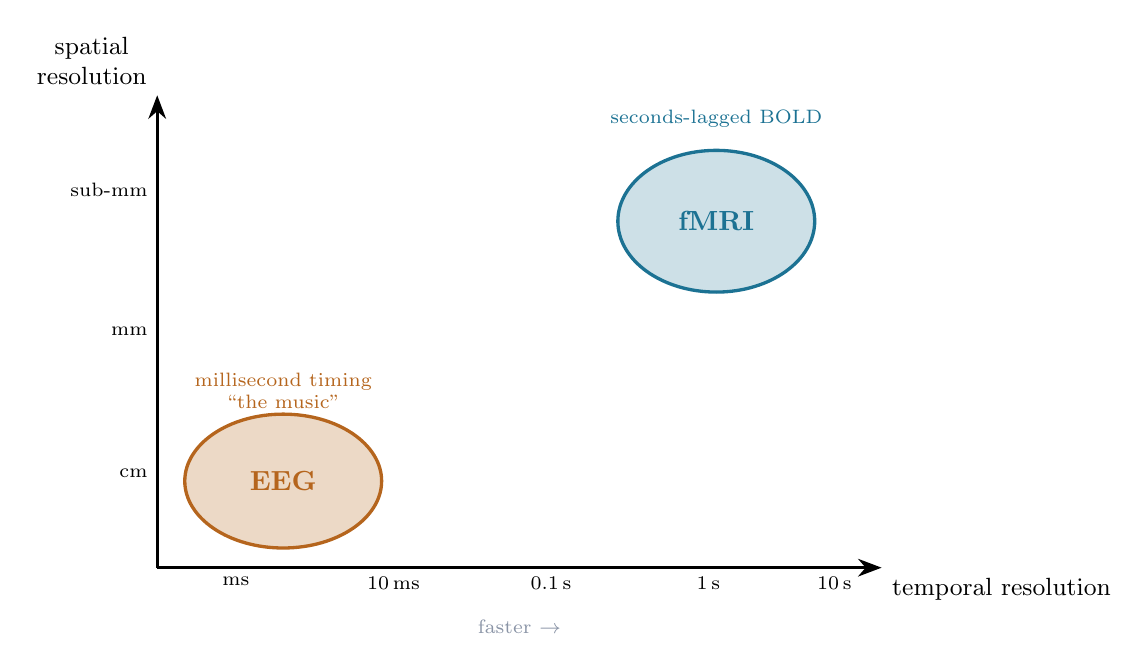
\begin{tikzpicture}[font=\sffamily]
  \draw[-{Stealth[length=3mm]},line width=1pt] (0,0) -- (9.2,0) node[below right,font=\small] {temporal resolution};
  \draw[-{Stealth[length=3mm]},line width=1pt] (0,0) -- (0,6.0) node[above left,font=\small,align=center] {spatial\\ resolution};
  % axis ticks (log-ish, conceptual)
  \foreach \x/\t in {1/ms,3/10\,ms,5/0.1\,s,7/1\,s,8.6/10\,s}{ \node[below,font=\scriptsize] at (\x,0) {\t};}
  \foreach \y/\t in {1.2/cm,3/mm,4.8/sub-mm}{ \node[left,font=\scriptsize] at (0,\y) {\t};}
  % fast axis annotation
  \node[font=\scriptsize,sbgrey] at (4.6,-0.75) {faster $\rightarrow$};
  % EEG region: fast temporal, coarse spatial (upper-left)
  \fill[sbaccent!25] (1.6,1.1) ellipse (1.25 and 0.85);
  \draw[sbaccent,line width=1.2pt] (1.6,1.1) ellipse (1.25 and 0.85);
  \node[sbaccent,font=\bfseries] at (1.6,1.1) {EEG};
  \node[font=\scriptsize,text=sbaccent,align=center] at (1.6,2.25) {millisecond timing\\ ``the music''};
  % fMRI region: slow temporal, fine spatial (lower-right)
  \fill[sbteal!22] (7.1,4.4) ellipse (1.25 and 0.9);
  \draw[sbteal,line width=1.2pt] (7.1,4.4) ellipse (1.25 and 0.9);
  \node[sbteal,font=\bfseries] at (7.1,4.4) {fMRI};
  \node[font=\scriptsize,text=sbteal,align=center] at (7.1,5.7) {seconds-lagged BOLD};
\end{tikzpicture}
\end{document}